\chapter{Évaluation du travail}
\label{ch:evaluation}
Après près d'une centaine d'heures de travail, il est nécessaire de prendre du recul.
Mon expérience de ce projet est globalement positive même s’il ne s'est pas déroulé sans accrocs.

Des développeurs séniors se sont déjà cassés sur ce problème, mais j'avais bon espoir de réussir en bénéficiant de leur expérience.

\section{Autocritique}
\label{sec:autocritic}

\paragraph{}
À Altissia, les membres de l'équipe IT sont tous des spécialistes et je ne fais pas exception.
Ma spécialité est le développement d'application côté \gls{g-server}.
Au cours de ce projet, j'ai essayé d'acquérir des connaissances sur des technologies avancées et je peux me vanter d'avoir ajouté quelques cordes à mon arc.

\paragraph{}
Le développement de l'interface utilisateur m'a par contre donné beaucoup de fil à retordre et j'ai complètement dépassé mes estimations de temps de travail.
La création d'un composant personnalisé pour glisser et déposer des fichiers m'a pris plus de cinq fois le temps prévu.
Avec le recul, je pense que j'aurai dû simplifier cette fonctionnalité-là.

\paragraph{}
Enfin, je suis content d'avoir exploré le langage de programmation Python.
J'ai par contre honte d'avoir consacré autant de temps à une fonctionnalité qui n'était pas nécessaire et a été finalement abandonné et l'on ne m'y reprendra plus.
Cela m'a été autorisé, car c'était mon temps libre que je gaspillais.

\subsection{L'élaboration du cahier des charges}
\label{subsec:specs}

\paragraph{}
La réalisation d'un cahier des charges est un exercice auquel je ne suis pas habitué et auquel je devrai encore consacrer du temps.

\begin{figure}[ht]
    \centering
    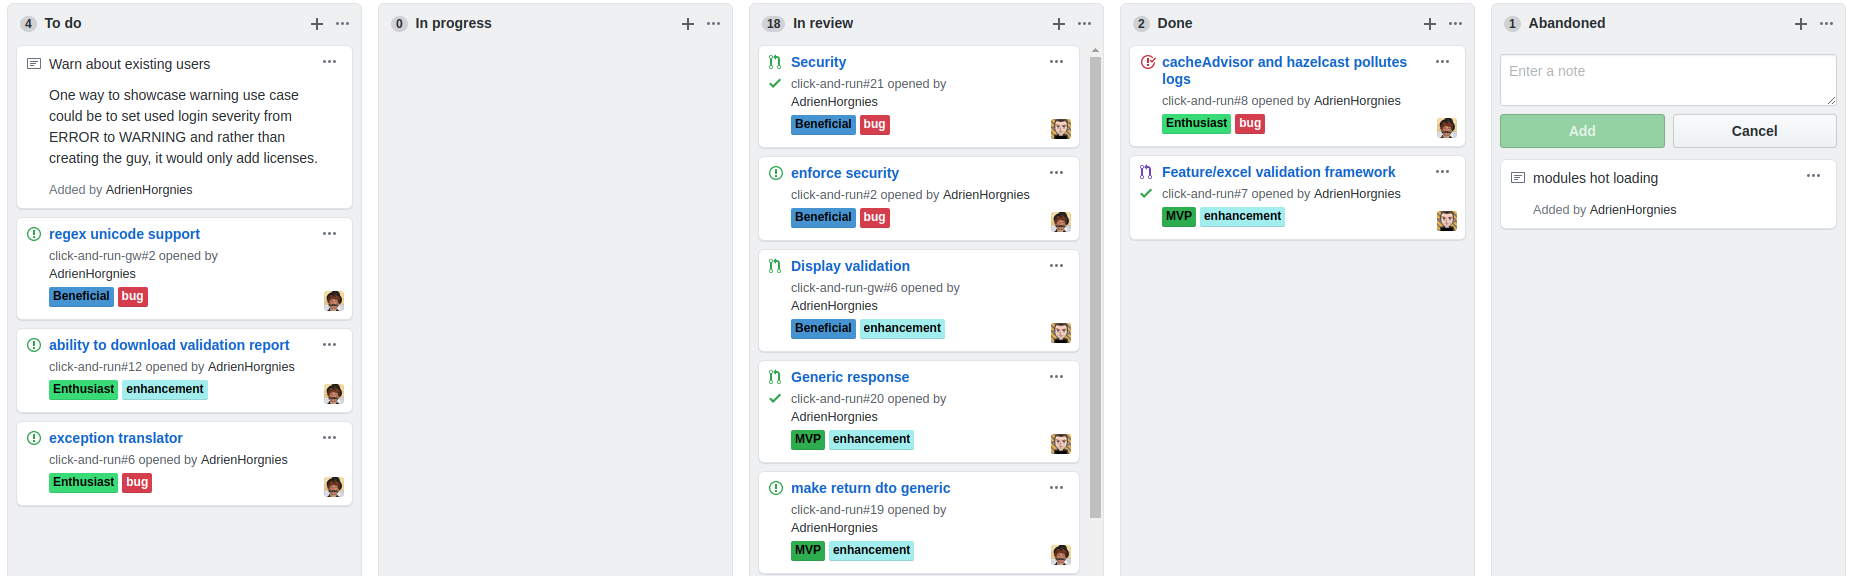
\includegraphics[width=1\textwidth]{images/github-project.png}
    \caption{La page de gestion de projet que j'ai mise en place sur GitHub}
    \label{fig:github-project}
\end{figure}

\paragraph{}
Mon équipe travaille selon les principes \gls{g-agile} et organise le travail interne avec le logiciel de suivi de projets Jira.
J'ai reproduit un comportement similaire avec le système de suivi de projets de Github (voir figure \ref{fig:github-project}).
Ce tableau modélise mieux mon expérience de développement que le présent cahier des charges.

\paragraph{}
En ayant écrit un cahier des charges, je suis passé de l'autre côté du tableau et j'ai enfilé la casquette de chef de projet.
Cela m'a ouvert les yeux sur beaucoup de difficultés auxquelles je ne dois pas faire face au quotidien.
Je pense par exemple à la transformation d'un ensemble chaotique de fonctionnalités en un planning de travail applicable.

\subsection{La conduite de l'analyse}
\label{subsec:analyse-is-hard}

\paragraph{}
J'ai déjà participé à la conception de plusieurs sites web et j'ai pu me passer de l'analyse de beaucoup d'éléments.

Les deux éléments principaux qui ont occupé mon travail d'analyse sont l'architecture des différents services et le système de modules.

\paragraph{}
Dans un premier temps, je ne parvenais pas à saisir les difficultés qui me bloquaient pour proposer une solution à la fois adaptée au problème d'Altissia et généralisable pour être distribuées à toutes personnes ayant un problème similaire.

Mes cours d'\gls{a-uml} étant un peu loin, je me suis replongé dans un livre: UML 2.5 par la pratique\cite{roques_uml_2018}.
Mes connaissances en la matière à nouveau aiguisées, j'ai pu proposer différents schémas à mon directeur technique.
Nous avons finalement modifié une des solutions que j'avais proposée pour arriver à la solution de la figure \ref{fig:detailed-archi}.

\paragraph{}
Le système de modules était le nerf de la guerre.
Toutes les solutions précédentes avaient fini en code spaghetti\fnmark{}.
\fntext{Le code spaghetti est code de très mauvaise qualité dont la structure est incompréhensible. Il est généralement le résultat d'ajout successif de code sans intégration réfléchie ou cohérente dans la base de code existante.}

J'ai développé des solutions partielles et j'ai schématisé les prochaines étapes en parallèle.
Cette approche itérative m'a permis de mieux cerner les problématiques en jeu et de mieux les schématiser.
Les diagrammes m'ont alors indiqué de quel côté attaquer le problème.

J'ai résolu de nombreux obstacles en cassant les couplages que je pouvais observer sur mes diagrammes.

La première solution complète que j'ai proposée n'était pas exactement telle que vue dans le diagramme \ref{fig:class-diagram-full} vu dans la sous-section, \ref{subsec:class-diagram} mais elle m'a permis d'y aboutir.

\subsection{La réalisation}
\label{subsec:realisation}

\paragraph{}
La partie de la réalisation du projet qui m'a pris le plus de temps a été l'apprentissage de nouvelles connaissances.

J'en ai beaucoup appris sur la réflexion, la généricité et la programmation par annotation.
J'ai dû faire plusieurs tests pour mettre en place le patron de conception de la stratégie et ce fut le troisième essai qui fut fructueux.
De plus, j'ai approfondi mes connaissances dans le \gls{g-framework} \Gls{g-spring}.

\paragraph{}
J'ai pu mettre en oeuvre de nombreuses compétences acquises lors de mon bachelier.
Si je devais en mettre une en avant, c'est la compétence d'acquérir de nouvelles compétences.

\paragraph{}
Les professeurs de l'IFOSUP nous le rappellent sans cesse, le métier de développeur se réinvente continuellement.
Le développeur de demain ne fera pas le même travail que le développeur de demain.

\section{Appréciation du client}
\label{sec:client-loves-me}

La cheffe de projet Sophie Roekhaut est satisfaite du résultat et se réjouit à l'idée du temps qu'elle va gagner sur un tas de tâches récurrentes.
Elle aurait par contre espéré que le projet aboutit plus rapidement.
Le projet auquel est dédié cet outil est en bonne voie et le contenu de cours publié sur base des données produites par Click-and-Run a passé tous les tests qualitatifs, ce qui n'était généralement pas le cas lorsque l'on utilisait les anciens outils.

De plus, elle est très optimiste par la future adoption de cet outil par le service du support et du service commercial.
Le service des linguistes l'a déjà adopté et attend son déploiement avec impatience.
Ils pourront exécuter en quelques secondes eux-mêmes des tâches pour lesquelles un développeur devait dédier plusieurs heures par le passé.

